%\vspace*{-1em}\section{A Taxonomy of Model Transfer RL}\label{sec:trl}
\section{A Taxonomy of Model Transfer RL}\label{sec:trl}
Now, we formally define the Model Transfer RL problem and derive a taxonomy of settings encountered in MTRL.

\subsection{MTRL: Problem Formulation}
Let us assume that we have access to a set of source MDPs $\mathcal{M}_s \triangleq \{\mu_i\}_{i=1}^m$. The individual MDPs can belong to a finite or infinite but compact set depending on the setting. For example, for tabular MDPs with finite state-actions, this is always a finite set. Whereas for MDPs with continuous state-actions, the transitions can be parameterised by real-valued vectors/matrices, corresponding to an infinite but compact set.
Given access to $\mathcal{M}_s$, we want to find an optimal policy for an unknown target MDP $\mdp^*$ that we encounter while deploying RL in the wild.
At each step $t$, we use $\mathcal{M}_s$ and the data observed from the target MDP $D_{t-1} \triangleq \{ s_0, a_0, s_1, \ldots, s_{t-1}, a_{t-1}, s_t\}$ to construct an estimate of $\mdp^*$, say $\hat{\mdp}^t$. Now, we use $\hat{\mdp}^t$ to run a model-based planner, such as \textsc{ValueIteration} or \textsc{RiccatiIteration}, that leads to a policy $\pol^t$. After completing this planning step, we interact with the target MDP using $\pol_t$ that yields an action $a_t$, and leads to observing $s_{t+1}, r_{t+1}$. We update the dataset with these observations: $D_t \triangleq D_{t-1} \cup \{a_{t}, s_t\}$. Here, we assume that all the source and target MDPs share the same reward function $\mathcal{R}$. We do not restrict the state-action space of target and source MDPs. %$\mathcal{S}_{\mathrm{target}} \times \mathcal{A}_{\mathrm{target}}$

Our goal is to compute a policy ${\pol}^t$ that performs as close as possible with respect to the optimal policy $\pol^*$ for the target MDP as the number of interactions with the target MDP $t\rightarrow \infty$.
This allows us to define a notion of regret for MTRL: $R(\mdp^{*}, \pol_t) \triangleq V_{\mdp^{*}}^{*}-V_{\mdp^{*}}^{\pol_t}$. Here, $\pol_t$ is a function of the source models $\mathcal{M}_s$, the data collected from target MDP $D_t$, and the underlying MTRL algorithm.
The goal of an MTRL algorithm is to minimise $R(\mdp^{*}, \pol_t)$.
For the parametric policies $\pol_{\theta}$ with $\theta \in \Theta \subset \mathbb{R}^d$, we can specialise the regret further for this parametric family: $R(\mdp^{*}, \pol_{\theta_t}) = V_{\mdp^{*}}^{\pol{\theta^*}}-V_{\mdp^{*}}^{\pol_{\theta_t}}$. For example, for LQRs, we by default work with linear policies. We use this notion of regret in our theoretical and experimental analysis.

%\cdcomment{Big picture: You do not define the model transfer problem at all. What is the criterion for a good transfer? Performance should depend on (a) the source MDPs (b) the target MDP (c) the number of episodes / horizon in the target MDP. Are you then comparing against the oracle policy of the target MDP? The mechanics of the transfer only seem to relate to (a) and (b)}

%\vspace*{-1em}\subsection{Three Classes of MTRL Problems}\vspace*{-.5em}
\subsection{Three Classes of MTRL Problems}
We begin by illustrating MTRL using Figure~\ref{fig:trl}. In the figure, the source MDPs $\mathcal{M}_s$ are depicted in red. This green area is the convex hull spanned by the source models $\mathcal{C}(\mathcal{M}_s)$. The target MDP $\mdp^{*}$, the best representative within the convex hull of the source models $\mdp$, and the estimated MDP $\hat{\mdp}$ are shown in blue, yellow, and purple, respectively. %The main takeaway of this figure is the location of the true model $\mdp^{*}$ relative to the source models. 
If the target model is \emph{inside} the convex hull, we call it a \textbf{realisable} setting. whereas If the target model is outside (as in Figure~\ref{fig:trl}), then we have a \textbf{non-realisable} setting.

Figure~\ref{fig:trl} also shows that the total deviation of the estimated model from the target model depends on two sources of errors: (i) realisability, i.e. how far is the target MDP $\mu^*$ from the convex hull of the source models $\mathcal{C}(\mathcal{M}_s)$ available to us, and (ii) estimation, i.e. how close is the estimated MDP $\hat{\mdp}$ to the best possible representation $\mdp$ of the target MDP. In the realisable case, the realisability gap can be reduced to zero, but not otherwise. This approach allows us to decouple the effect of the expressibility of the source models and the goodness of the estimator.
\setlength{\textfloatsep}{4pt}%
\begin{figure}
    \centering
    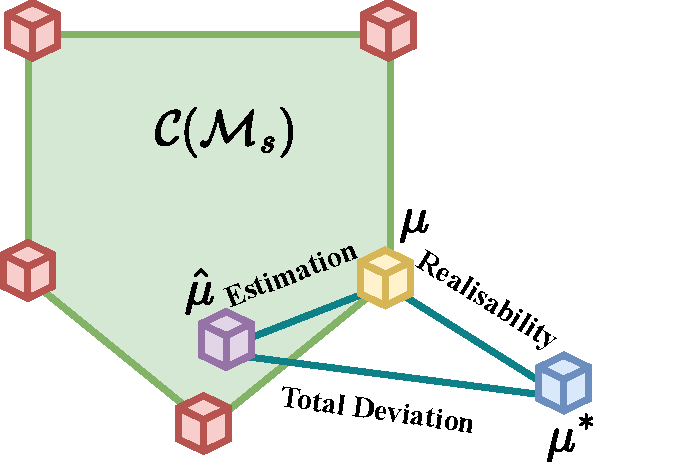
\includegraphics[width=0.35\paperwidth]{img/TRL.pdf}
    \caption{An illustration of the MTRL setting. The source models $\mathcal{M}_s$ are the red boxes. The green area is the convex hull $\mathcal{C}(\mathcal{M}_s)$ spanned by the source models. The target MDP $\mdp^{*}$ is displayed in blue, and the best proxy model is contained in the convex hull $\mdp$ in yellow. Finally, the estimator of the best proxy model $\hat{\mdp}$ is shown in purple.}
    \label{fig:trl}
\end{figure}
\iffalse
(a) \textbf{Finite and realisable setting:}  If the true model $\mdp^{*}$ is part of the convex hull spanned by the source models $\mdp^{*} \in \mathcal{C}(\mathcal{M}_s)$ and the optimisation over the possible models is taken directly over the source models, that is, the selected model $\hat{\mdp} \in \mathcal{M}_s$. Relating back to Figure~\ref{fig:trl}, optimisation is taken directly over the red boxes. 

(b) In the second setting, \textbf{infinite and realisable setting} the true MDP is again part of the convex hull $\mdp^{*} \in \mathcal{C}(\mathcal{M}_s)$. However, now the optimisation is taken over the convex hull. In Figure~\ref{fig:trl} this corresponds to the green area. 

(c) Thirdly, in the \textbf{infinite and non-realisable} setting, we have no guarantee the true MDP is part of the convex hull. In fact, it can be arbitrarily far away. Finally, we describe how we obtain (near)-optimality under the TRL framework and the measure of \emph{regret}.
\fi

%\subsection{MLE for The Three Classes of MTRL}
Now, we further elaborate on these three classes and the corresponding implications of performing MLE.

\textbf{I. Finite and Realisable Plausible Models.}\label{subsec:finite}
If the true model $\mdp^{*}$ is one of the target models, i.e. $\hat{\mdp} \in \mathcal{M}_s$, we have to identify the target MDP from a finite set of plausible MDPs. Thus, the corresponding MLE involves a finite set of parameters, i.e. the parameters of the source MDPs $\mathcal{M}_s$. We compute the MLE $\hat{\mdp}$ by solving the optimisation problem:
\begin{equation}
    \hat{\mdp} \in \underset{\mdp' \in \mathcal{M}_s}{\arg\max} \, \log \mathbb{P}(D_t \, | \, \mdp'), D_t \sim \mdp^{*}.
\end{equation}
This method may serve as a reasonable heuristic for the TRL problem, where the target MDP is the same as or reasonably close to one of the source MDPs. However, this method will potentially be sub-optimal if the target MDP is too different from the source MDPs. %, it may also suffer performance degradation in the case where true MDP lies within the compact set spanned by the convex hull of the source MDPs, see Figure~\ref{fig:trl}. 
Even if $\mdp^{*}$ lies within the convex hull of the source MDPs (the green area in Figure~\ref{fig:trl}), this setting restricts the selection of a model to one of the red boxes. Thus, this setting fails to leverage the expressiveness of the source models as MLE allows us to accurately estimate models which are also in $\mathcal{C}(\mathcal{M}_s)$. Thus, we focus on the two settings described below.

\textbf{II. Infinite and Realisable Plausible Models.}\label{subsec:realisable}
In this setting, the target MDP $\mdp^{*}$ is in the convex hull $\mdp^{*} \in \mathcal{C}(\mathcal{M}_s)$ of the source MDPs. Thus, for Class I, we extend the parameter space considered in MLE to an infinite but compact parameter set. 

Let us define the convex hull as $\mathcal{C}(\mathcal{M}_s) \triangleq \{\mdp_1 w_1 + \hdots + \mdp_m w_m \, | \, \mdp_i \in \mathcal{M}_s, w_i \geq 0, i=1, \hdots, m, \sum_{i=1}^m w_i = 1\}$. Then, the corresponding MLE problem with the corresponding likelihood function is %given by:
\begin{equation}\label{eq:realisable}
    \hat{\mdp} \in \underset{\mdp' \in \mathcal{C}(\mathcal{M}_s)}{\arg\max} \, \log \mathbb{P}(D_t \, | \, \mdp'), D_t \sim \mdp^{*}.
\end{equation}
%{\color{red}For example, for tabular MDPs, the target MDP can always be expressed in the convex hull.} I don't think that's true
Since $\mathcal{C}(\mathcal{M}_s)$ induces a compact subset of model parameters $\mathcal{M}' \subset \mathcal{M}$, Equation~\eqref{eq:realisable} leads to a \emph{constrained maximum likelihood estimation problem}~\citep{aitchison1958maximum}. It implies that if the parameter corresponding to the target MDP is in $\mathcal{M}'$, it can be correctly identified. In the case where the optimum lies inside, we can use constrained MLE to accurately identify the true parameters given enough experience from $\mdp^{*}$. This approach allows us to leverage the expressibility of the source models completely. However, $\mdp^{*}$ might lie outside or on the boundary. Either of them may pose problems for the optimiser.

\textbf{III. Infinite and Non-realisable Plausible Models.}\label{subsec:non-realisable}
This class is similar to Class II with the important difference that the true parameter $\mdp^*$ is outside the convex hull of source MDPs $\mathcal{C}(\mathcal{M}_s)$, and thus, the corresponding parameter is not in the induced parameter subset $\mathcal{M}'$. This key difference means the true parameters cannot be correctly identified. 
Instead, the objective is to identify the best proxy model $\mdp \in \mathcal{M}'$. The performance loss for using $\mdp$ instead of $\mdp^{*}$ is intimately related to the model dissimilarity $||\mdp^{*}-\mdp||_1$. This allows us to describe the limitation of expressivity of the source models by defining the \textit{realisability gap}: $\epsilon_{\mathrm{Realise}} \triangleq \min_{\mdp \in \mathcal{C}(\mathcal{M}_s)}\|\mdp^{*}-\mdp\|_1 $. The realisability gap becomes important while dealing with continuous state-action MDPs with parameterised dynamics, such as LQRs. %something described in more detail in Section~\ref{sec:bounds}.

\iffalse
\subsection{Performance Metric of MTRL}

The \emph{regret} associated with a policy $\pol$ is defined in terms of its potential loss compared to a clairvoyant agent knowing the optimal policy $\pol^{*}$, within the same parameter class. If $V_{\mdp^{*}}^{*} = \underset{\theta \in \Theta}{\sup}\, V_\mdp^{\pol_{\theta}}$, then the regret $R(\mdp^{*}, \pol_\theta) = V_{\mdp^{*}}^{*}-V_{\mdp^{*}}^{\pol_\theta}$. We make the conscious decision of only comparing against the optimal policy of the same parameter class for simplicity. The policy obtained using the model-based planning method for LQR problems gives a linear policy. 
\fi